\begin{MyChapter}{Játékfejlesztés webes alapokon}	
	% leírni mi lesz a fejezetben
	% először szót kell ejteni néhány témáról: html5, stb: melyek a webes környezet miatt kapcsolódnak a játékfejlesztéshez is.
	Az alábbi fejezetben a webes fejlesztés témakörével fogunk foglalkozni, általánosságban, és játékfejlesztés terén egyaránt. Szót fogok ejteni a webes fejlesztéshez használatos népszerű technológiákról, például a HTML5-ről, vagy a webes projektekhez leggyakrabban használt programnyelvekről, mint a JavaScript illetve a TypeScript.
	Miután röviden ismertetem a JavaScript programnyelvet, írni fogok a JavaScriptet támogató keretrendszerekről is, ezenkívül olvashatunk majd a keretrendszer nélküli játékfejlesztésről, az ahhoz használatos API-kat is beleértve. A fejezet végén pedig a játékmotorok közül néhányat picit részletesebben ismertetni fogok.

	\begin{MySection}{Webes fejlesztés}
		% kialakulása, néhány általános dolog
		Az internet fejlődésével a böngészőkben játszható játékok nem csak helyet kaptak, de szinte a legnagyobb közönséghez jutottak el. A hozzáférésük sokkal könnyebb, mint a boltokban megvásárolt játékoknak, hiszen szimplán csak egy webcímre szükséges ellátogatni, majd magában a böngészőben zajlik a játékmenet. Napjainkban pedig az eszközeink nagy részén már rendelkezésre áll egy böngésző. Ezen felül a szociális hálózatok elterjedése szintén felgyorsította a böngészős játékok egyre több emberhez való eljutását.
		\cite{browser_games}
		\cite{html5_games}
		% irodalomjegyz.->
 		% https://en.wikipedia.org/wiki/Browser_game
		% https://www.awwwards.com/current-state-and-the-future-of-html5-games.html
		% irodalomjegyz.->
		% https://docs.microsoft.com/en-us/archive/msdn-magazine/2015/march/game-development-a-web-game-in-an-hour
		
		Azonban a böngészők erőforrásai kifejezetten korlátozottak voltak, komplexebb alkalmazásokhoz már nem biztosítottak elég funkciót. Ezért a fejlesztők különböző cégek által készített plug-in-eket, programokat használtak, mint például a Microsoft Silverlight, vagy az Adobe Flash. Ezek a kiegészítések már komolyabb grafikus tartalom megjelenítésére voltak képesek, viszont az összes használónak szükséges telepítenie a megfelelő plugin-t. 
		
		Kijelenthetjük tehát, hogy a mai modern kornak és a webes szabványoknak köszönhetően, ma már böngészőbe épülő plugin-ek nélkül is képesek vagyunk modern hardveresen gyorsított számítógépes grafika, illetve a felhasználói elvárásokat kielégítő szintű játékok készítésére.
	\end{MySection}

	\begin{MySection}{HTML5}
		% mi ez, miért jobb mint ami eddig volt
		% html5
		A HTML5 egy új, átdolgozott változata a HTML (Hypertext Markup Language) régebbi verzióinak.
		Azonban a HTML5 nem csak szimplán egy átdolgozott változat, hanem új elemekkel, tulajdonságokkal is bővült, valamint egyes elemek új funkciók elérését is biztosítják.
		
		Létrehozásának a fő célja a fentebb említett funkcióknak az egységesítése volt, anélkül, hogy a felhasználóknak különböző plugin-eket kellene használniuk webes applikációkhoz, hogy megfelelően működjenek az egyes elemek a böngészőben.
		A funkciók szabványosítása folyamatosan zajlik, így bár már most is megfelelő felületet nyújt a webes játékok, alkalmazások számára, a jövőben még ennél is népszerűbbé válhat.
		\newline \newline
		A HTML5 néhány főbb jellemzője, előnye:
		\begin{itemize}
			\item Pluginoktól való függetlenséget nyújt, így a felhasználók számára sokkal könnyebben hozzáférhető.
			\item Reszponzív, hasonló felhasználói élményt nyújt különböző típusú eszközökön.
			\item Mobilokon kevesebb sávszélesség használat szükséges hozzá, mint a sima HTML-hez, ezáltal a mobilok akkumlátora is tovább tarthat.
			\item Egyéb különféle technológiák is könnyedén használhatóak együtt a HTML5-tel. (Például: PHP, MySQL)
		\end{itemize}

		A HTML5 és JavaScript alapú technológiák előkelő helyet foglalnak el platformfüggetlenség terén, viszont fontosnak tartom megjegyezni, hogy ezzel a technológiával egy összetettebb, nagyobb adattartalommal rendelkező játékot (ma még legalábbis) nem feltétlenül érdemes elkészíteni, mert könnyedén megizzaszthatja nem csak az átalgos felhasználók számítógépeit, hanem akár a modernebb gépeket is.
		\cite{html5_future}
		\cite{html5}
		% irodalom ->
		% https://www.topnotchdezigns.com/reasons-html5-future/
		% https://developer.mozilla.org/en-US/docs/Web/Guide/HTML/HTML5
	\end{MySection}

	\begin{MySection}{JavaScript}
		%  mi ez, miért jó
		%  kialakulása
		A JavaScript (röviden: JS) egy kis erőforrás-igényű, dinamikus, objektum-orientált programozási nyelv, mely lehetőséget nyújt a fejlesztők számára a weboldalaikba való komplexebb dolgok implementálására. Amennyiben olyan weblapról beszélünk, amely nem statikus tartalommal rendelkezik, hanem interaktív tartalom is megtalálható rajta, akár 2D-s vagy 3D-s animáció, stb., abban az esetben valószínűsíthető, hogy JavaScriptet is tartalmaz az oldal. Ezenkívül, bár webes tartalmaknál használják a leggyakrabban, számos webböngészőn kívüli környezetben is alkalmazható. A nyelvet eredetileg 1996-ban fejlesztették ki, azóta sokat változott, a szintaxisa közelebb került a Java programozási nyelvhez. Az ECMA (Európai informatikai és kommunikációs rendszerek szabványosítási szövetsége) először 1997 és 1999 között szabványosította ECMAScript néven.
		\cite{javascript_prog_wiki}
		\cite{javascript_oktatoanyag}
		\cite{javascript_pros_cons}
		% irodalom ->
		% https://developer.mozilla.org/en-US/docs/Learn/JavaScript
		% https://hu.wikipedia.org/wiki/JavaScript
		% https://developer.mozilla.org/hu/docs/Web/JavaScript
		% https://hu.wikipedia.org/wiki/Ecma_International
		% https://wiki.prog.hu/wiki/JavaScript
		% https://data-flair.training/blogs/advantages-disadvantages-javascript/
		\newline \newline
		A JavaScript főbb jellemzői:
		
		\begin{itemize}
			\item A futási környezete többnyire egy webböngésző.
			\item Lehetőséget ad az interaktivitásra. (Ezalatt a felhasználó által megvalósított események kezelhetőségére gondoljunk.)
			\item A legtöbb böngészővel kompatibilis, emiatt népszerű is.
			\item Lehetővé teszi a böngésző irányítását.
			\item A megjelenített tartalmak átalakítására is lehetőséget ad.
			\item A kiszolgáló tehermentesítését is elősegíti: Űrlapküldés esetén küldéskor megvizsgálhatja, hogy az összes űrlapmező ki van-e töltve. Amennyiben nincs, a kliens oldalon fel tudja hívni a felhasználó figyelmét erre.
			\item Sokoldalú, mivel alkalmas front-end és backend fejlesztésre, valamint weboldalak vagy webapplikációk tesztelésére egyaránt.
		\end{itemize}
		A játékipar tekintetében egyik legnépszerűbb alkalmazása, az összepárosítása a HTML5 canvas elemével. Rengeteg játékmotor készült ennek a segítségével.
		
		Összességében elmondhatjuk, hogy a JavaScript szinte mindenhol futtatható, rengeteg helyen alkalmazzák, és ezalatt a front-end valamint a back-end mellett a mobil, az asztali, illetve a hibrid alkalmazásokat is érthetjük. A nyelv kifejezetten népszerű, folyamatosan fejlődik, a webfejlesztés egyik vezető programnyelve és ez feltehetőleg még hosszú ideig így is marad.
		\cite{javascript_future}
		% irodalomjegyzék ->
		% https://www.creative-tim.com/blog/web-development/javascript-future-learn-javascript/
		% TODO megnézni h van e vmi hasznos ebben https://www.freecodecamp.org/news/future-of-javascript
	\end{MySection}

	\begin{MySection}{TypeScript}
		% mi ez, miért jó
		% kialakulása
		A TypeScript szintén egy objektum-orientált nyelv, tulajdonképpen a JavaScript típusokkal, osztályokkal, és egyéb hasznos funkciókkal kibővített változata. Tehát minden, amit JavaScript-ben megtehetünk, az TypeScript-ben is lehetséges, továbbá egy működő JavaScript kódot átvihetünk TypeScript kódba, az ott is le fog futni, a futási időben való viselkedés pedig nem fog változni, még akkor sem, ha a TypeScript úgy érzékeli, hogy a kód típushibákat tartalmaz. Fordítás során a TypeScript fájlok JavaScripté konvertálódnak át. A nyelvet a Microsoft készítette. Érdemes észrevennünk, hogy a TypeScript-ben található típusok, osztályok, privát illetve publikus láthatóságok, stb. ellenőrzése csak fordítási időben történik meg, futásidőben nem garantált.
		A TypeScript megjelenése előtt a JavaScript programozók gyakran követtek el típushibákat, még akár szimpla elgépelések miatt is. Ezen hibák kiküszöbölésével azonban a TypeScript hatékonyabbá teheti a JavaScript fejlesztést, nagyobb projektek esetében is.
		\cite{typescript}
		% irodalom->
		% https://www.typescriptlang.org/
		\newline \newline
		A nyelv főbb jellemzői tehát a következők:
		\begin{itemize}
			\item Objektum-orientált programozási nyelv.
			\item Teljesen nyílt forráskódú.
			\item A fordító a TypeScript forráskódból JavaScript kódot generál.
			\item Operációsrendszer független valamint böngészőfüggetlen.
			\item Egy már meglévő JS kódot fel tudunk használni TypeScriptben, tehát felülről kompatibilis a JavaScript nyelvvel.
		\end{itemize}
		% ESLint TSLint (PMD, Chechstyle Java esetén)
	\end{MySection}

	\begin{MySection}{Általános célú JavaScript keretrendszerek}
		% nem játékfejlesztéshez használatos keretrendszerek
		Korábban már volt szó a keretrendszerekről, melyeket játékfejlesztésre használhatunk, azonban természetesen léteznek ezeken túl is keretrendszerek. A JavaScript úgymond "beépített" funkcióinak alkalmazása nem elég effektív, ezért előbb-utóbb szükségünk lehet valamilyen libraryre vagy keretrendszerre. A továbbiakban általános célú JavaScript keretrendszerekről lesz szó.
		Ha úgy döntünk, hogy használni szeretnénk például egy JS keretrendszert, rengeteg széles körben elterjedt, népszerű opció áll a rendelkezésünkre, és mindnek megvan a saját előnye, valamint hátránya, attól függően, hogy mi a fő célunk vele: például front-end, backend fejlesztés, vagy tesztelés. Emiatt nehéz lehet eldönteni, hogy vajon melyik is lenne tökéletes választás számunkra. A döntésben esetlegesen segítségünkre lehetnek a különféle keretrendszerek népszerűségével kapcsolatos statisztikák. Ehhez rendelkezésünkre állhatnak különböző források az interneten (például a következő weboldal: \url{https://bestofjs.org/})
		Az említett weblapon nyomon követhetjük a felhasználók általi használat alapján a napi, heti, havi vagy akár az éves legnépszerűbb keretrendszereket.
		\cite{best_js_framework}
		% irodalom --->
		% https://www.lambdatest.com/blog/best-javascript-framework-2020/
		
		% TODO angular, react esetleg leírni
		Néhány kimondottan elterjedt keretrendszer például a Vue.js, React és az Angular. Ezek egyébként ebben a sorrendben 2017-ben az akkori év első három leghasználtabb JS keretrendszerei voltak a weboldal alapján, melyről fentebb szó volt.
		Az említett keretrendszerek közül az egyikről, konkrétabban a Vue.js-ről egy rövid bemutatást is olvashatunk alább.
		
		\begin{MySubSection}{Vue.js}
			A Vue.js egy nyílt forráskódú JavaScript keretrendszer, amely 2014-ben látott napvilágot, és azóta is az egyik legkedveltebb keretrendszerek közé tartozik. A nyílt forráskódúság azért lehet fontos szempont, mert ilyen esetben a keretrendszerek az elterjedt operációs rendszereken szinte biztosan elérhetőek. A frontend, illetve a fullstack fejlesztői pályára készülőknek hasznos lehet megismerkedniük a Vue-val.
			\cite{js_framework}
			% irodalom --->
			% https://skillcrush.com/blog/what-is-a-javascript-framework/
			A keretrendszert Vue-ként is emlegetik, kiejtésének hangzása az angol "view", azaz magyarul "nézet" szóra hasonlít, ez akár utalhat is arra, hogy MVVM (modell-nézet-nézetmodell) mintát követ, tehát lényegében szétválasztja a grafikus felhaszálói felületet (vagy rövidebben a megjelenítést), valamint az üzleti logikát.
			A Vue képességei közül érdemes megjegyeznünk az újrafelhasználható komponensek építését, illeve azoknak a kommunikációját.
			\cite{vue_bevezetes}
			\cite{vue_pros_cons}
			% irodalom ->
			% https://www.altexsoft.com/blog/engineering/pros-and-cons-of-vue-js/
			% https://ithub.hu/blog/post/Bevezetes-a-Vuejs-keretrendszerbe
			Ezenkívül mellette szól még, hogy a Vue fokozatosan implementálható a kódunkba, tehát ha egy már létező projektben például más technológiával oldottunk meg valamit, akkor ezeket kis részenként is lecserélhetjük. Azonban az sem feltétlenül gond, ha nem szeretnénk teljes mértékben lecserélni, képes együttműködni például jQuery-vel, vagy más egyéb JS könyvtárakkal.
			Összességében, a Vue.js szépen felépített, könnyedén megtanulható keretrendszer, amit szerintem mindenképp ajánlatos kipróbálni.
			\cite{vue_alapozo}
			% irodalom ->
			% https://thebojda.medium.com/vue-js-alapoz%C3%B3-8be3a4db812d
		\end{MySubSection}
	\end{MySection}

	\begin{MySection}{Webes játékfejlesztés}
		% TODO a címet esetleg módosítani?
		%  szükséges egyéb dolgok pl.: grafikai pakkok (al-al-fejezetek), hangok, texturák, objektumok
		% TODO ide még másról szükséges lenne írnom?
		
		Webes játékkészítéskor szükségünk lehet bizonyos plusz elemekre a játékunk elkészítéséhez, gondolhatunk itt textúrákra, felhasználói felülethez (GUI) szükséges elemekre, animációkra, audióra, stb. Amennyiben nem saját magunk szeretnénk elkészíteni ezeket a plusz dolgokat, az interneten rengeteg megfelelő grafikai pakk, asset (magyarul: forrás) található meg, rendelkezésünkre állnak mind fizetősek, mind ingyenesek. Ezek tehát lehetnek textúrák, hangok, animációk, sprite-ok, stb., két- és három dimenziós alkalmazásokhoz egyaránt. 
		
		A dimenziók száma meghatározó szerepet játszik abban, hogy milyen vizualizációs formát választunk a játékunk megjelenítéséhez. Mint később szó lesz róla, a szakdolgozat részeként egy 2D-s játékot készítek el, emiatt a három dimenziós grafikai megjelenítésekre most nem igazán fogok kitérni a fejezetben.
		
		% Tile-map
		Két dimenziós grafika esetén kimondottan elterjedt a Tile-Map alapú megjelenítési technika. Egyébként ehhez a módszerhez is számos asset lehet a segítségünkre az internetről. Az eljárás lényege, hogy kijelzőt virtuálisan azonos méretű úgynevezett Tile-okra bontjuk, és mivel ezeket a mezőket újra és újra felhasználjuk a felhasználó számára megjelenítendő háttérhez, ezért a memóriában helyet spórolhatunk meg azzal, hogy csak egyszer töltjük be az egyes tile-okat. A vizualizációs forma előnyei között tudható még, hogy akár nagyobb távolságra is valós időben lehetséges az útkeresés és az útvonal elaborálása, valamint (amennyiben az adott alkalmazáshoz elegendő a kisebb szintű vizuális komplexitás) viszonylag könnyedén kivitelezhető vele az ütközésvizsgálat.
		\cite{mileff}
		% irodalom ->
		% https://users.iit.uni-miskolc.hu/~mileff/grafika/Grafika_programozasa_jegyzet_v0.66_Mileff_P.pdf
		A már elkészített és szétdarabolt tile-ok összességét Tileset-nek nevezzük. A Tileset-et leggyakrabban egy külön képben szokás tárolni. (Például így: \myref{fig:tileMap:tileSet} ábra)
		\cite{tileset}
		% irodalom ->
		% http://higherorderfun.com/blog/2012/05/20/the-guide-to-implementing-2d-platformers/
		\begin{figure}[H]
			\centering
			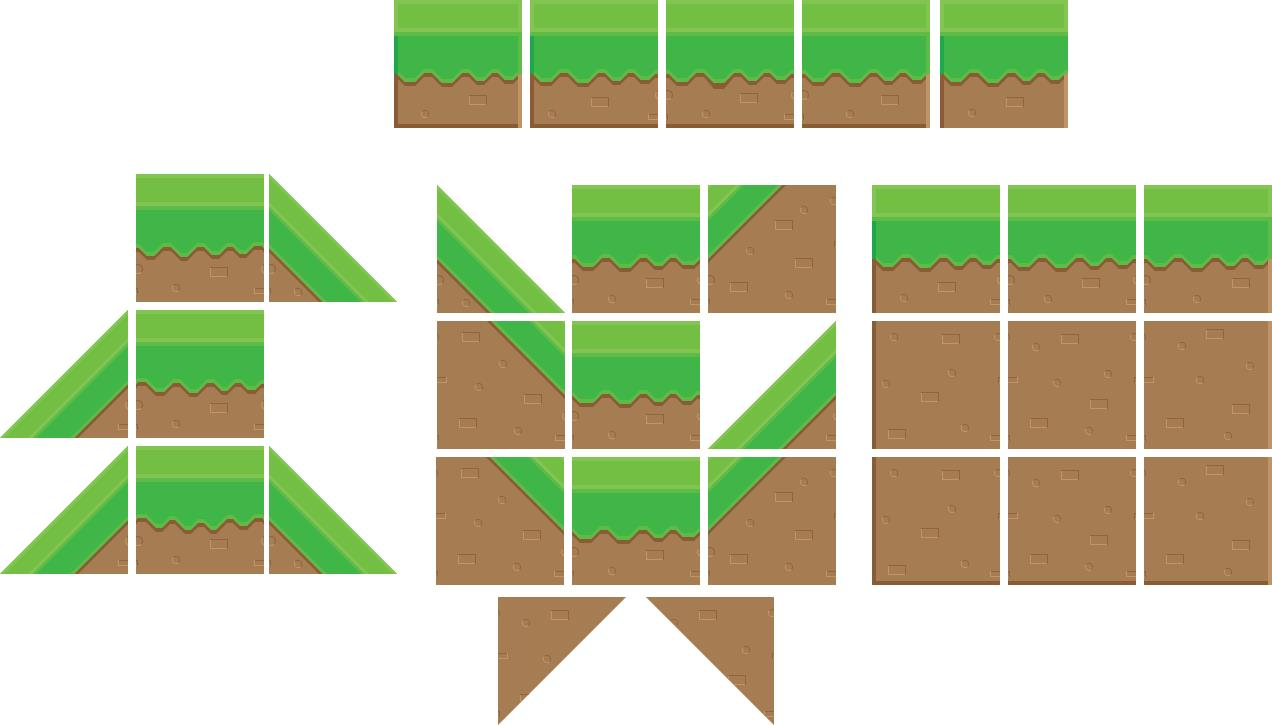
\includegraphics[scale=0.25]{kepek/tileMap/TileSet.png}
			\caption{Platform játékhoz alkalmas tileset}
			\label{fig:tileMap:tileSet}
		\end{figure}
	
		A Tile-Map alapú megjelenítésre a legalkalmasabb játéktípusok között vannak a felülnézetes, a puzzle, vagy például a platformer játékok. (A fentebbi tileset és egyéb elemek használatával példa a megjelenítési technikára: \myref{fig:tileMap:tileMapPreview} ábra)
		
		\begin{figure}[H]
			\centering
			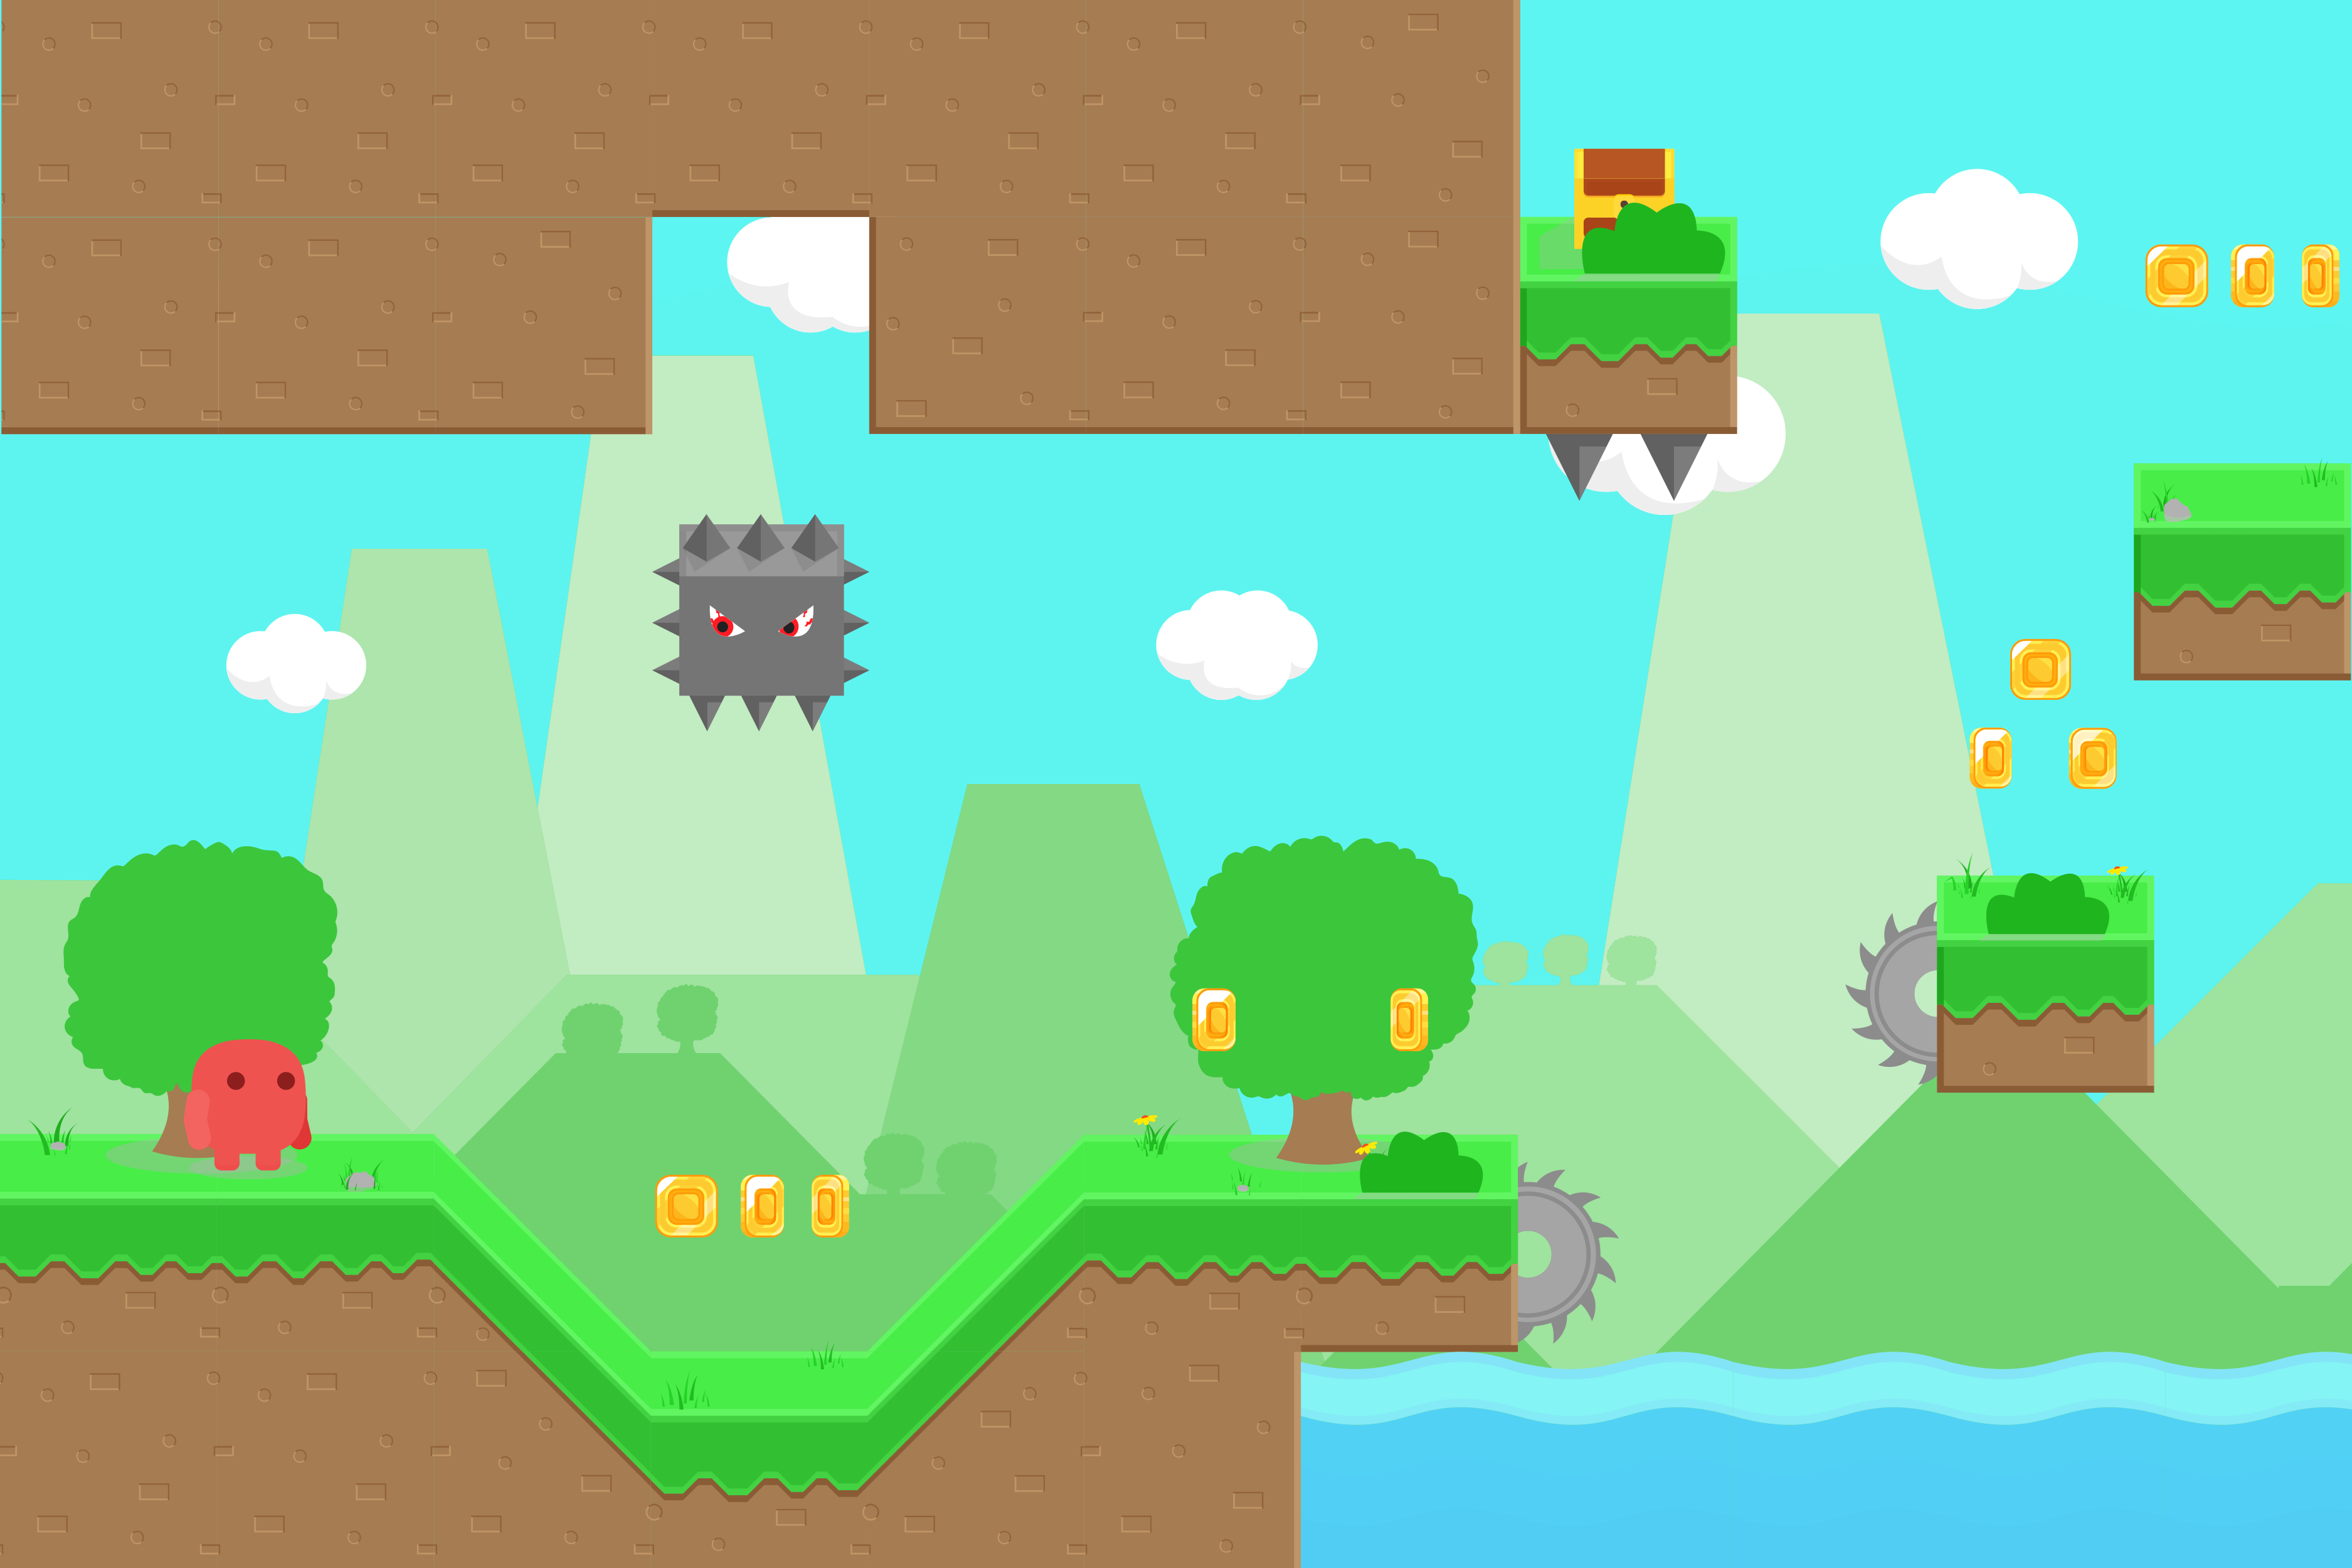
\includegraphics[scale=0.35]{kepek/tileMap/TileMapPreview.png}
			\caption{Példa tilesettel létrehozott platform játékra}
			\label{fig:tileMap:tileMapPreview}
		\end{figure}
		% irodalom ->
		% https://bayat.itch.io/platform-game-assets
		
		% keretrendszerrel vagy nélküle
		A fentebb említettek mellett, egy játék elkészítése előtt még az a feladat is vár ránk, hogy eldöntsük azt, hogy keretrendszerrel vagy pedig anélkül fogunk fejleszteni. 
		Mindkét módnak megvan a saját előnye és hátránya, a mi dolgunk, hogy mérlegeljünk, számunkra az adott projekthez melyik lenne alkalmasabb.
		\cite{tile_map}
	\end{MySection}

	\begin{MySection}{Webes játékfejlesztés keretrendszerek nélkül}
		% "pure js"-ben
		A \myref{Játékfejlesztés keretrendszerek nélkül} fejezetben leírtak természetesen webes fejlesztésnél is érvényesek.
		Alapvetően keretrendszerek nélküli játékfeljesztés alatt az úgynevezett "pure JavaScript"-et értjük. (A pure angol szó jelentése magyarul: tiszta.)
		Tehát ideértendő az, amikor csak JavaScriptet használunk a fejlesztéshez. 
		A webes játékfejlesztés esetében a webböngészőben való grafikus megjelenítéshez alapvetően két API-t használhatunk: a Canvast, valamint a WebGL-t, melyekről alább láthatunk egy-egy rövid ismertetőt.
		
		% canvas
		\begin{MySubSection}{Canvas-ról röviden}
			A Canvas API tehát egy grafikai rajzoló módszert biztosít JavaScript, és a html canvas elemével. Nagyrészt 2D-s grafikára fókuszál.
			Rengeteg dologra használhatjuk, melyek között szerepelnek a következők:
			\cite{canvas_api}
			% irodalom ->
			% https://developer.mozilla.org/en-US/docs/Web/API/Canvas_API
			\begin{itemize}
				\item Animáció
				\item Játék grafika
				\item Adatok szemléltetése
				\item Fotószerkesztés
				\item Valós idejű videófeldolgozás
			\end{itemize}
			% TODO átolvasni h a canvas jó-e így
		\end{MySubSection}
		
		% webgl
		\begin{MySubSection}{WebGL-ről röviden}
			A WebGL (Web Graphics Library, magyarul: webalapú grafikus könyvtár) tehát egy JavaScript API, amely interaktív két dimenziós (röviden: 2D), illetve három dimenziós (röviden: 3D) grafikát tud ábrázolni bármely kompatibilis webböngészőben, plugin-ek használata nélkül.
			\cite{webgl01}
			\cite{webgl02}
			% irodalom->
			% https://matebalazs.hu/api-application-programming-interface.html
			% https://hu.wikipedia.org/wiki/Alkalmaz%C3%A1sprogramoz%C3%A1si_fel%C3%BClet
			% https://developer.mozilla.org/en-US/docs/Web/API/WebGL_API
			% https://en.wikipedia.org/wiki/WebGL
			% https://en.wikipedia.org/wiki/Cross-platform_software
			% https://www.khronos.org/webgl/wiki/Getting_Started
			
			Számos előnyt felsorolhatunk, hogy miért lehet érdemes használnunk a WebGL-t, a teljesség igénye nélkül megemlítenék párat közülük:
			\begin{itemize}
				\item Ingyenes a használata.
				\item Az OpenGL szolgált alapjául, emiatt azon fejlesztőknek, akik OpenGL-t használtak már, ismerős, egyszerű lehet a WebGL alkalmazása. 
				\item Cross-platform, avagy platformfüggetlen, többféle platformra is implementálható.
				\item Lehetővé teszi a hardveres gyorsítós böngészős játékokat (a felhasználó eszközétől függően).
				\item Nincs szükség plugin-ek használatára.
				\item Egy olyan környezet, amelyben a 3D grafika ellenőrzése egyszerű, könnyen debug-olható.
				% irodalom->
				% https://www.quora.com/What-are-the-pros-and-cons-of-WebGL
			\end{itemize}
		\end{MySubSection}
		
	\end{MySection}

	\begin{MySection}{Webes játékfejlesztés keretrendszerekkel}
		% keretrendszerek miért jók
		% felsorolni (tovább bontani al-al-fejezetekre ha megoldható)
		% megemlíteni melyik miért jó, miben más, használatuk, esetleg kipróbálás, személyes tapasztalatok
		% összehasonlítás eredménye / összegzése az előzőnek
		% dönteni melyiket használom -> Phaser 3
		
		Keretrendszerekkel való (nem webes) játékfejlesztésről beszéltünk már, azonban a webes játékfejlesztés terén sincs sok különbség annak tekintetében, hogy a használatukkal hatékonyabban, gyorsabban lehetünk képesek egy játék elkészítésére, kimondottan kezdőként könnyebb lehet a fejlesztés játékmotor alkalmazásával, mint anélkül.
		
		Amennyiben valaki játékfejlesztés előtt áll, és úgy dönt, hogy keretrendszert fog használni az alkalmazás elkészítéséhez, még rengeteg átgondolnivalója van, például abban a tekintetben, hogy melyik motort fogja használni. Fontos, hogy megtaláljuk a célunkhoz legmegfelelőbb keretrendszert. A választást rengeteg dolog befolyásolhatja, például az elkészíteni kívánt játék grafikája, a preferált programnyelv, vagy hogy mennyire nehéz egy-egy keretrendszer használatának elsajátítása, satöbbi. A lehetőségek felméréséhez segítség lehet például egy-egy tömör összefoglalást átolvasni az egyes motorokról, vagy ha az időnk engedi kipróbálni, tapasztalatokat gyűjteni róluk, majd azután összevetni őket.
		
		\begin{MySubSection}{Játékmotorok összehasonlítása}
			Arra az elhatározásra jutottam, hogy a szakdolgozatom részeként elkészítendő játékot egy keretrendszer segítségével fogom elkészíteni, ezért a most következő részben különféle játékfejlesztéshez használható HTML5 alapú játékmotorokat fogok összehasonlítani röviden, hogy egy kis áttekintést kapjunk néhány lehetséges motorral kapcsolatosan. Számomra most egyrészt az a fontos, hogy ingyenesen használható legyen a motor, másrészt, mivel 2D-s játékot szeretnék készíteni, az is lényeges, hogy egy erre jobban alkalmas keretrendszert használjak, ne pedig három dimenziós játékok fejlesztésére készített játékmotort. 
			Ezek a feltételek már önmagukban leszűkítették a szóba jöhető keretrendszerek körét, de az egyes motorok dokumentációit és a felhasználói véleményeket is figyelembe fogom venni a választás során. Végül négy játékmotor volt, amik szimpatikusabbak voltak, így jobban utánuk néztem, ezekről fogok pár szót írni, majd pedig eldönteni, hogy melyiket fogom használni a játék elkészítéséhez.
			\newline \newline
			A négy összehasonlítandó keretrendszer:
			
			\begin{itemize}
				\item \textit{ImpactJS}, \url{https://impactjs.com/}
				\item \textit{Modd.io}, \url{https://www.modd.io/}
				\item \textit{Construct 2}, \url{https://www.construct.net/en/construct-2/download}
				\item \textit{Phaser}, \url{https://phaser.io/}
			\end{itemize}
		\end{MySubSection}
	
		\begin{MySubSection}{ImpactJS Engine}
			Az ImpactJS egy olyan JavaScript játékmotor, amivel mobil és számítógép böngészőjében használható alkalmazásokat készíthetünk főképp 2D-s játékokat. A legtöbb népszerű böngészőt támogatja.
			Az motor egy saját level-editorral (magyarul: pályaszerkesztő) rendelkezik, aminek Weltmeister a neve, ennek a használatához egy saját webszerver működésére van szükség. Elsőre kissé bonyolultnak tűnt kezdőként, mert nincs nagy tapasztalatom webszerver használatával, és a funkciók nem működtek megfelelően az első pár próbálkozásnál. Pozitívum, hogy az ImpactJS oldalán és fórumain rengeteg kérdésre választ találtam. Node.js-el, valamint annak az impact-node package-ével sikerült működtetni az editort, a kisebb problémák leküzdése után, viszont ennél egyszerűbb megoldást találva, végül az EasyPHP Webszervert használtam, aminek a grafikus felülete felhasználóbarát, egyszerű. Az editor alapvetően egy üres pályát tölt be, egyetlen réteggel, amiben az entitások találhatóak (például az ellenfelek, NPC-k stb) ezután pedig új pályákat készíthetünk, és el is tudjuk menteni azokat. Az engine oldalán találhatók demo játékok, letölthető forráskódokkal, valamint tutoriál videó is, ezekben a nagyon alapokat találhatjuk meg. Emellett több olyan dokumentum is található, mely kifejezetten kezdőknek lehet segítség, egy-egy egész játék fejlesztésén vezetnek végig, azonban ezek már fizetősek. Alapvetően nem tűnik rossznak, viszont több, mint 6 éve nem volt semmilyen frissítés a keretrendszerhez, emiatt is vált pár éve ingyenessé maga a motor. Öszességében szimpatikus, és könnyen tanulhatónak tűnik, ami ellenben nem tetszik benne, hogy nem túl naprakész.
			\cite{impactjs}
			% irodalom ->
			% https://impactjs.com/
		\end{MySubSection}
			
		\begin{MySubSection}{Modd.io}
			A következő motor a Modd.io, amely böngészőből használható, letöltés nem szükséges, csak egy regisztráció, ezáltal a saját projektekhez, valamint az editorhoz is hozzáférést nyerünk. A játékokat, amit készítünk könnyedén publikálhatjuk, vagy továbbíthatjuk másnak, mivel gyorsan készíthető egy instant link, amit megnyitva más is kipróbálhatja az alkotást, ezt a „publikálást” természetesen bármikor leállíthatjuk. Ahhoz, hogy az alapokat elsajátítsuk, viszonylag rövid, lényegre törő oktató videók vannak fent a Modd.io honlapján, melyeket egyszerű követni, és ezáltal megtanulni velük a fontosabb alapvető dolgokat, persze a komplexebb problémák megoldásához már nem feltétlenül elegendő ez. Amikor elkezdünk készíteni egy új projektet, lehetőség van kiválasztani, hogy kezdőként vagy haladóként vagyunk ott, ettől függ, hogy az editorban minden tulajdonságot elérünk-e, mert kezdőként például leegyszerűsíti a felhasználói felületet. Azt is megadhatjuk, hogy milyen típusú játékot készítünk (például PVP, Tower defense, stb.), valamint az alap pálya kinézetét, stílusát, és csak ezek után kerülünk az editorba, ott pedig már kedvünkre alakíthatjuk a dolgokat.
			\cite{modd.io_official_website}
			% irodalom ->
			% https://www.modd.io/
			Ha több segítségre van szükségünk, Discord-on viszonylag gyorsan válaszolnak a kérdésekre, akár más felhasználók is készséggel segítenek, amennyiben tudnak.
			A motor elég naprakésznek tűnik, és felhasználóbarátnak, azonban az utóbbi miatt kissé korlátozottnak is érződnek számomra a lehetőségeink a fejlesztés során.
			Emellett a felhő-alapú technológia miatt, főleg biztonsági szempontokat figyelembe véve nem feltétlenül szimpatikus számomra, hiszen akár csak véletlenül egy biztonségi rés által, vagy pedig szándékosan is eltulajdoníthatják az egész munkánkat, vagy akár csak az ötleteinket.
		\end{MySubSection}
	
		\begin{MySubSection}{Construct 2}
			A Construct 2 egy különösképp 2D-s játékok fejlesztéséhez ajánlott keretrendszer, eseményalapú működésű. A motornak van egy ingyenes verziója, ami kevesebb lehetőséggel rendelkezik, mint a fizetős, de kezdésnek megfelelő, egyszerű, és részletes oktató anyagot mellékelnek hozzá, amit szintén ingyenesen elérhetünk. Felhasználóbarát megjelenése van, és ugyancsak számos platformon működik a kód változtatása nélkül.
			A Construct 2 már előre elkészített úgynevezett "viselkedésekkel" rendelkezik. Például található benne viselkedés mozgáshoz a billentyűzeten lévő nyilakkal, vagy egy adott elem (pl. a játékos) mozgásának követése is ilyen viselkedés, illetve annak a megoldását is tartalmazza, hogy ne tudjunk lemenni a pályáról, avagy az adott layer-ről. Mi magunk is elkészíthetnénk ezeket, viszont hasznos, hogy van lehetőség már előre elkészített viselkedések alkalmazására is.
			Mint ahogy fentebb már említettem, eseményalapú, így nem kell túl sokat kódolni egy alkalmazás elkészítéséhez, így kezdő programozók számára például sokkal egyszerűbb, átláthatóbb a használata.
			Létezik egyébként már a fejlettebb, újabb, Construct 3 is, viszont az már csak előfizetéses verzióval rendelkezik, valamint letölteni már nem feltétlenül kell, hanem böngészőn belül is lehet vele alkotni.
			A Construct 2-t azonban már nem fejlesztik tovább, hanem a Construct 3-mal dolgoznak csak, így egyre kevésbé modern az elődje.
			A szakdolgozatomhoz végeredményben nem szeretném használni, mert viszonylag korlátozottak benne a lehetőségek, főleg az ingyenes verziójában, illetve a dokumentációja sem annyira kimagasló, emellett mint korábban írtam ez sem kifejezetten naprakész motor.
			\cite{construct_2_manual}
			\cite{construct_2_javascript_sdk}
		\end{MySubSection}
			
		\begin{MySubSection}{Phaser}
			A Phaser 3 egy teljesen ingyenesen használható cross-platform játékmotor, nyílt forráskódú, kifejezetten két dimenziós játékok készítésére alkalmas. A fejlesztés JavaScripttel és TypeScripttel is kivitelezhető a motorral. Számomra ez azért lényeges, mert amennyiben lehetséges, TypeScriptet támogató keretrendszert szeretnék használni, mivel a típusok használata sok esetben megkönnyítheti a fejlesztést.
			A felhasználói vélemények nagyrészt pozitívak róla, amivel azok alapján kivetnivalók lehetnek, hogy bár a plugin támogatottsága nagyon jó, egyes pluginok fizetősek az ingyenes motor mellé. Ezzel szemben, eddig számomra úgy tűnik, hogy a fontosabbakat tartalmazza az ingyenes verzió is, így lehetségesnek tartom, hogy a pluginokkal kapcsolatos negatív vélemények oka az, hogy egy régebbi verzióhoz íródhattak.
			Egyszerűen tanulhatónak tűnik első benyomás alapján, rengeteg tutorial, útmutató van hozzá, apróbb példák, és egy-egy komplett játék fejlesztésén végigvezető könyvszerű dokumentumok egyaránt, magyarázatokkal. Azonban komplexebb példákat nem igazán mellékeltek hozzá.
			A hivatalos honlapjukon szereplő tutorialok közül kettőt elolvastam, illetve végigcsináltam, egyet JavaScriptben, egyet pedig TypeScriptben (ez gyakorlatilag 2 könyv: 69 és 102 oldalakkal). \cite{infinite_jumper} \cite{infinite_runner}
			% http://assets.ourcade.co/books/Infinite_Jumper_Phaser3_Modern_JavaScript.pdf
			% http://assets.ourcade.co/books/Infinite_Runner_Phaser3_TypeScript.pdf
			A kipróbálás után úgy gondolom, kezdők számára könnyen elsajátíthatóak az alapok, a telepítése egyszerű, nem igényel semmilyen külön beállítást, gyakorlatilag pár perc előkészület után már használható is.
			Szerintem kisebb projektek aránylag egyszerűen megvalósíthatóak vele.
			Viszonylag gyakran frissítik, így naprakésznek tűnik, és kifejezetten népszerűnek is.
			A dokumentációját azonban nem mondanám annyira jónak, mert csak az alapokra tér ki, bonyolultabb témákban szinte semmi útmutató nincs, és úgy általánosságban sem különösen részletezi a dolgokat. Az osztályokat leírja, hogy mire valók, de nincs összetettebb összefoglaló, hogy ha egy-egy adott dolgot szeretnénk csinálni, mit érdemes használni hozzá, illetve néhány metódus nincs is kifejtve, hogy hogyan használható, hanem csak fel van sorolva, hogy egy adott osztályban mely metódusok találhatóak. Így ha komplexebb, nehezebb dolgokat szeretnénk megvalósítani benne, más fórumokon nagyobb eséllyel találhatunk segítséget, vagy magunknak kell kikísérleteznünk a megoldást.
			
			% TODO ### phaser alapvető dolgait leírni: ###
			%mi az a scene (itt lenne a logika + a ui)
			%game
			%config
			%group
			%gameobject, sprite, image, +physics enabled versions
			%arcade / mattejs physics
			%spritesheet/imageatlas
			%- miért jó, miért jobb mint ha egyesével töltenénk be a képeket
			%-  gondolj itt a 4k*4k-s videókártya buffer méretere, amibe ha betöltünk egy ilyen pont beleillő képet amin több különböző dolog is van, sokkal gyorsabb csak az adott memóriában lévő képen pozíciót ugrani, mintsem külön másik képet betölteni a memóriába, főleg animációknál fontos ez a gyorsaság miatt.
			%fizika overlap vs collision különbség ütközés vizsgálatkor
			%- overlap átefdést néz, nem tolja el egymástól az objektumokat, a collision igen, így nekünk érdemesebb az overlapot használni hiszen a lövedékeinknek nem kellene eltolni az ellenfelet, leglaábbis nem volt cél, ez viszotn felvet egy másik poblémát, hogy kezelni kell ha egyszerre több dologgal kerül "átfedésbe" a lövedék, illetve kezelni kell, hogy ha ugyan azzal a dologgal kerül többször is átefedésbe, pl egy lövedék ha van penetration-je ne tudja ugyan azt az ellenfelete többször is sebezni.
		\end{MySubSection}
			
		\begin{MySubSection}{A fejlesztéshez kiválasztott játékmotor}		
			Összességében a fentebb felsorolt keretrendszereket összevetve számomra a Phaser tűnik a legszimpatikusabbnak, ezért a szakdolgozatom részeként elkészítendő játékot ennek a játékmotornak a segítségével fogom elkészíteni. Természetesen ezzel nem azt szeretném mondani, hogy a többi motort nem is érdemes használni, hiszen csak felületesen próbáltam ki őket. Ha mindegyikkel egy egész, hasonló projekt fejlesztését végigcsináltam volna, meglehet, hogy más eredményre jutottam volna, azonban sajnos erre most nem volt idő.
			Az esetlegesen felmerülő problémákat, negatív vagy épp pozitív véleményeket melyek a fejlesztés során felmerülnek, megfogalmazódnak bennem, a későbbiekben részletezni fogom. Ezenkívül a játék elkészülte után azt is leírom, hogy javasolnám-e másnak ilyen jellegű projekthez a válaszott motort, vagy sem.
		\end{MySubSection}

	\end{MySection}
	
\end{MyChapter}